% Aurora 战队 RoboMaster 雷达站 2026 赛季传承文档
% 编译: xelatex Aurora战队雷达站传承文档.tex
% 字体约定: 正文宋体(Noto Serif CJK SC), 标题黑体(Noto Sans CJK SC), 全文黑白
\documentclass[11pt,a4paper,fontset=none]{ctexart}
\usepackage[margin=2.4cm]{geometry}
\usepackage{graphicx}
\usepackage{booktabs}
\usepackage{tabularx}
\usepackage{array}
\usepackage{enumitem}
\usepackage{float}
\usepackage{caption}
\usepackage[hidelinks]{hyperref}
% ---- 字体设置: 正文宋体, 标题黑体 ----
\setCJKmainfont{Noto Serif CJK SC}
\setCJKsansfont{Noto Sans CJK SC}
\setCJKmonofont{Noto Sans CJK SC}
\setCJKfamilyfont{zhhei}{Noto Sans CJK SC}
\providecommand*{\heiti}{\CJKfamily{zhhei}}
\ctexset{
  section/format={\heiti\Large\bfseries},
  subsection/format={\heiti\large\bfseries},
}
\setmonofont{DejaVu Sans Mono}[Scale=0.85]
\captionsetup{font=small}
\newcommand{\code}[1]{\texttt{#1}}
\setlist{nosep}
\title{\heiti\textbf{Aurora 战队雷达站传承文档}}
\author{赵书彤 \\[2pt] \small QQ：19732579198}
\date{2026 年 9 月}

\begin{document}
\maketitle

\tableofcontents

%======================================================
\section{T-DT 开源代码概况}

上游代码为东北大学 T-DT 实验室 2025 赛季开源项目（\code{T-DT\_Radar-main}）。
其 README 说明：``本项目提供了除串口、相机驱动、模型训练外雷达站的全部功能''，
即感知、融合、标定与地图可视化可直接使用，但串口通信、相机图像采集与推理模型三部分缺失。
代码分为 \code{tdt\_vision}（标定、检测、解算、推理）、\code{lidar}（配准、聚类、动态点）、
\code{fusion}（卡尔曼跟踪、地图显示）、\code{interface}（消息定义）、\code{livox\_driver}（雷达驱动）、
\code{utils}（回放与转换脚本）六个部分，各模块实现较为基础，仅满足实验室环境下的回放验证，
与实际参赛要求存在较大差距。

硬件方面，原版为 Livox Avia、海康 CH-120-10UC、i7-12700KF 与 RTX A4000$\times$2；
本战队为 Livox Mid-70 激光雷达、海康 MV-CS060 相机（6mm 镜头），整机为惠普暗影精灵 10
笔记本电脑（RTX 4060 显卡），另由本人购置 1TB 固态硬盘用于雷达站数据存储。
该硬件配置满足雷达站的使用需求，后续提升主要取决于代码的完善。

%======================================================
\section{改造总览}

\begin{table}[H]
\centering\small
\begin{tabularx}{\textwidth}{lrrX}
\toprule
文件 & T-DT 原版 & 本项目 & 主要改动 \\
\midrule
detect.cpp & 334 & \textbf{999} & 增加 SR 超分、3D 框、5 槽位输出、机器人号映射 \\
kalman\_filter.cpp & 206 & \textbf{1488} & 增加 Hungarian 匹配、id\_score 身份置信、行为预测 \\
debug\_map.cpp & 285 & \textbf{728} & 增加盲区预测点、双倍易伤自动触发 \\
resolve.cpp & 141 & \textbf{329} & 增加 HeightGrid 地形高度修正 \\
localization.cpp & 187 & \textbf{483} & CPU GICP 改为 CUDA ICP \\
cluster.cpp & 84 & \textbf{250} & 扩充聚类与目标过滤逻辑 \\
calibrate.cpp & 190 & \textbf{451} & 标定流程按 2026 场地重写 \\
\midrule
\multicolumn{4}{l}{\textbf{完全新增：}radar\_serial\_node.cpp（裁判系统串口）、camera/hik.cpp（相机驱动）、}\\
\multicolumn{4}{l}{rm\_control\_panel（Qt 控制面板）、databag\_tool（录包）、create\_sr\_onnx.py 等（超分模型脚本）}\\
\bottomrule
\end{tabularx}
\caption{从 T-DT 开源到参赛系统的核心文件改动统计。}
\end{table}

%======================================================
\section{各模块改造说明}

\subsection{相机驱动}
接入海康 MV-CS060 的 SDK（\code{src/tdt\_vision/camera/MV\_SDK}），编写 \code{hik.cpp}
完成图像采集、曝光控制与内参加载，发布至 \code{camera\_image} 话题；
夜间曝光参数保存于 \code{config/camera\_driver\_night.yaml}。

\subsection{检测 detect}
在原 YOLO 检测与装甲板分类基础上：增加 SR 超分（先低分辨率快检，再对感兴趣区域超分放大，
脚本 \code{utils/create\_sr\_onnx.py}、\code{utils/pb2onnx\_sr.py}）；利用外参叠加 3D 框显示；
按 2026 规则将装甲板数字映射至 5 个槽位（1 英雄、2 工程、3 步兵三号、4 步兵四号、6 哨兵；
2026 赛季无步兵五号与空中单位），写入 \code{DetectResult} 的 \code{red\_x/blue\_x} 数组。
槽位填写存在同号覆盖缺陷，见 \S4.2。

\begin{figure}[H]
  \centering
  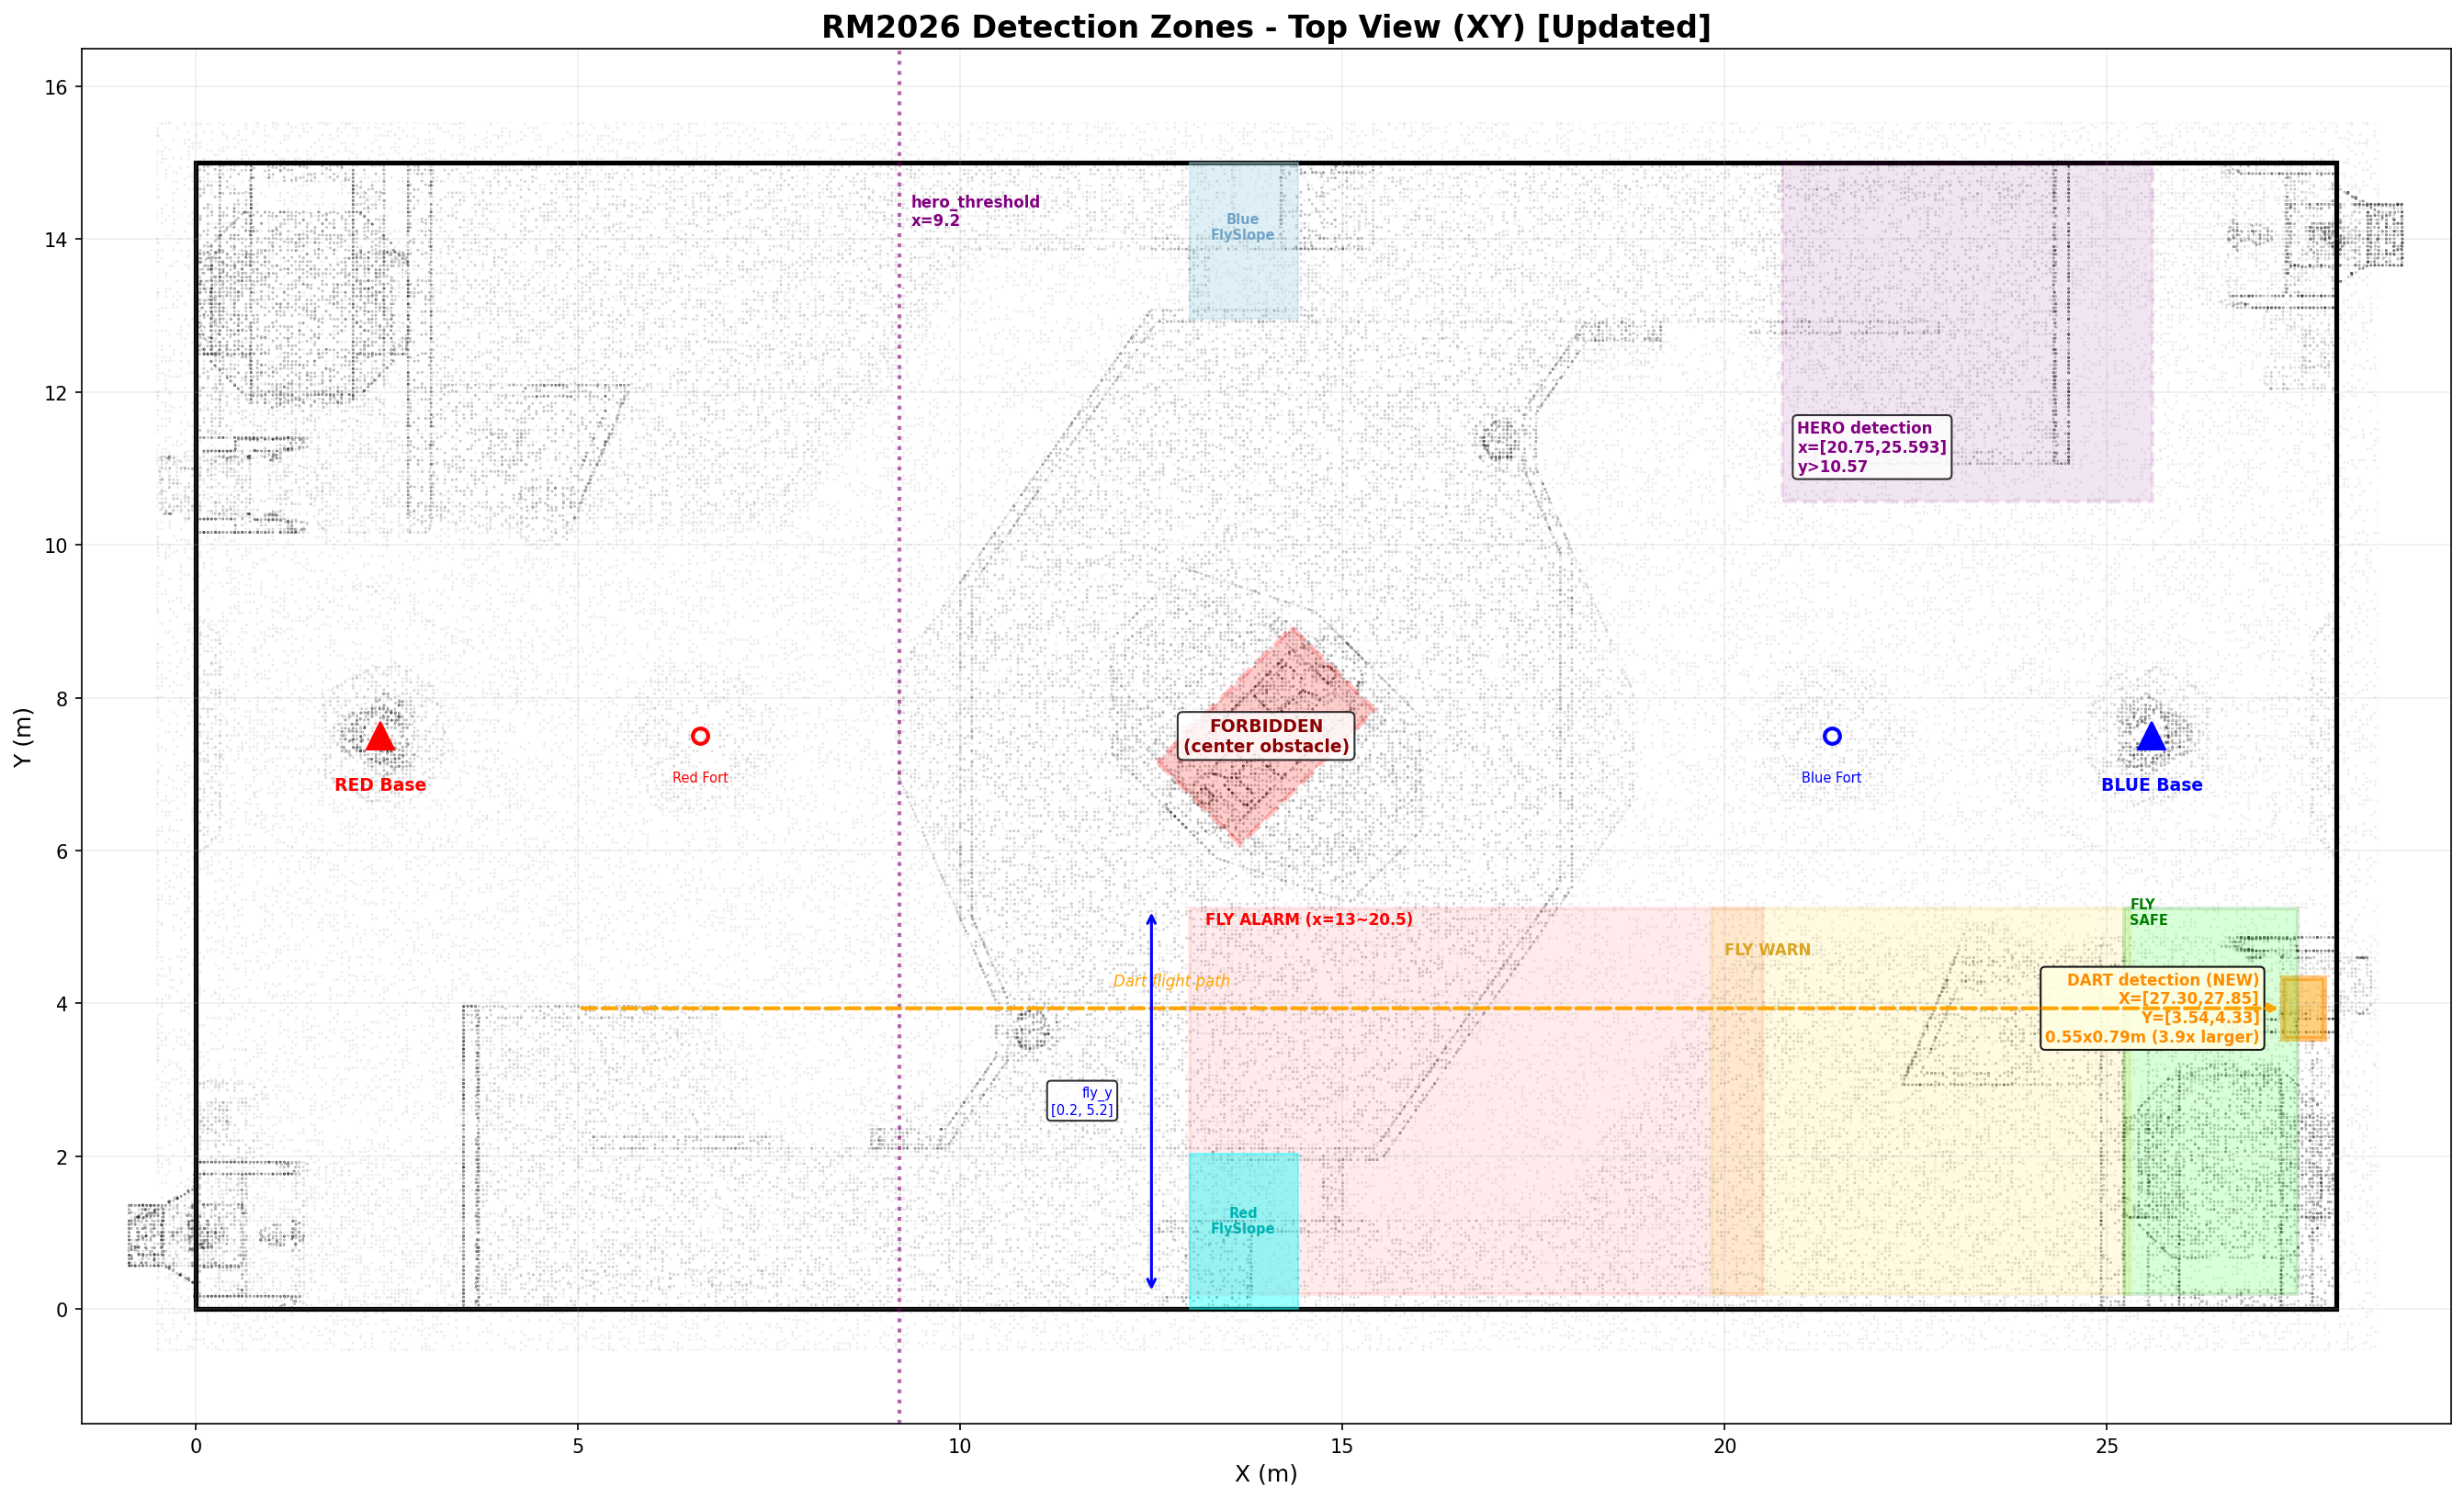
\includegraphics[width=0.82\textwidth]{figs/detection_zones.png}
  \caption{RMUC 2026 检测与判定区域划分（俯视 XY 平面）：英雄检测区、飞镖区、
  飞坡警戒/安全区与中央高台禁发区等。}
\end{figure}

\subsection{融合 kalman\_filter}
增加 Hungarian 匹配（KF 轨迹与新检测结果做二分图最优匹配）、id\_score 身份置信
（仅装甲板数字识别稳定时赋值）、行为分类预测（目标进入盲区后按 CHARGING/TUNNEL/OUTPOST/
ASSEMBLY 四类预测位置，重新可见后接管）；融合结果经 \code{/radar2sentry} 发送至串口节点。

\subsection{标定 calibrate}
五点标定流程按 2026 场地重做（我方堡垒、我方前哨、敌方基地、敌方前哨、中央高塔），
外参分色保存为 \code{config/\{red,blue\}/out\_matrix\_*}，检测窗口 3D 框用于验证贴合程度。
雷达被搬动后外参即失效，局间必须重新标定。

\begin{figure}[H]
  \centering
  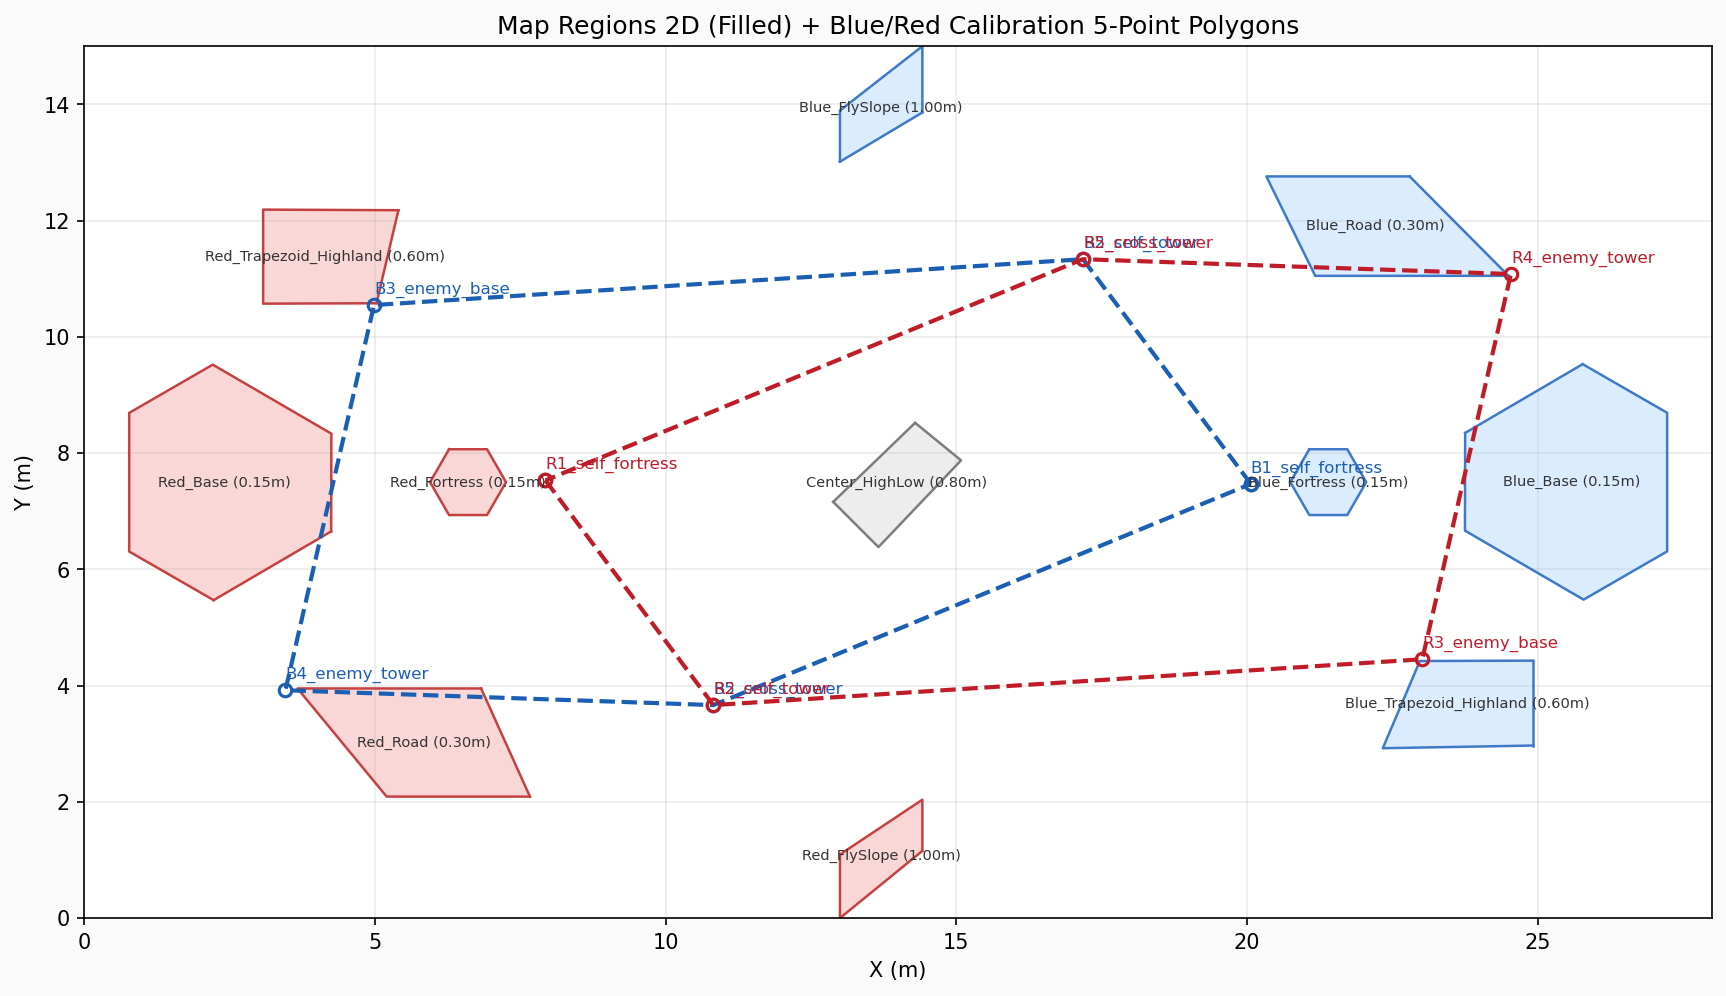
\includegraphics[width=0.8\textwidth]{figs/calib_points.png}
  \caption{地图区域划分与红蓝双方五点标定路径（我方堡垒 $\to$ 我方前哨 $\to$
  敌方基地 $\to$ 敌方前哨 $\to$ 中央高塔）。}
\end{figure}

\subsection{解算 resolve 与配准 localization}
resolve 增加 HeightGrid 地形修正：预计算 \code{config/map/field\_mesh.bin} 网格高度，
像素投影至世界坐标时查询实际地面高度修正。localization 由 CPU GICP 改为 CUDA ICP
（\code{cuda\_icp.h}），地图更换为 2026 赛季场地扫描点云 \code{config/map/map.pcd}。

\begin{figure}[H]
  \centering
  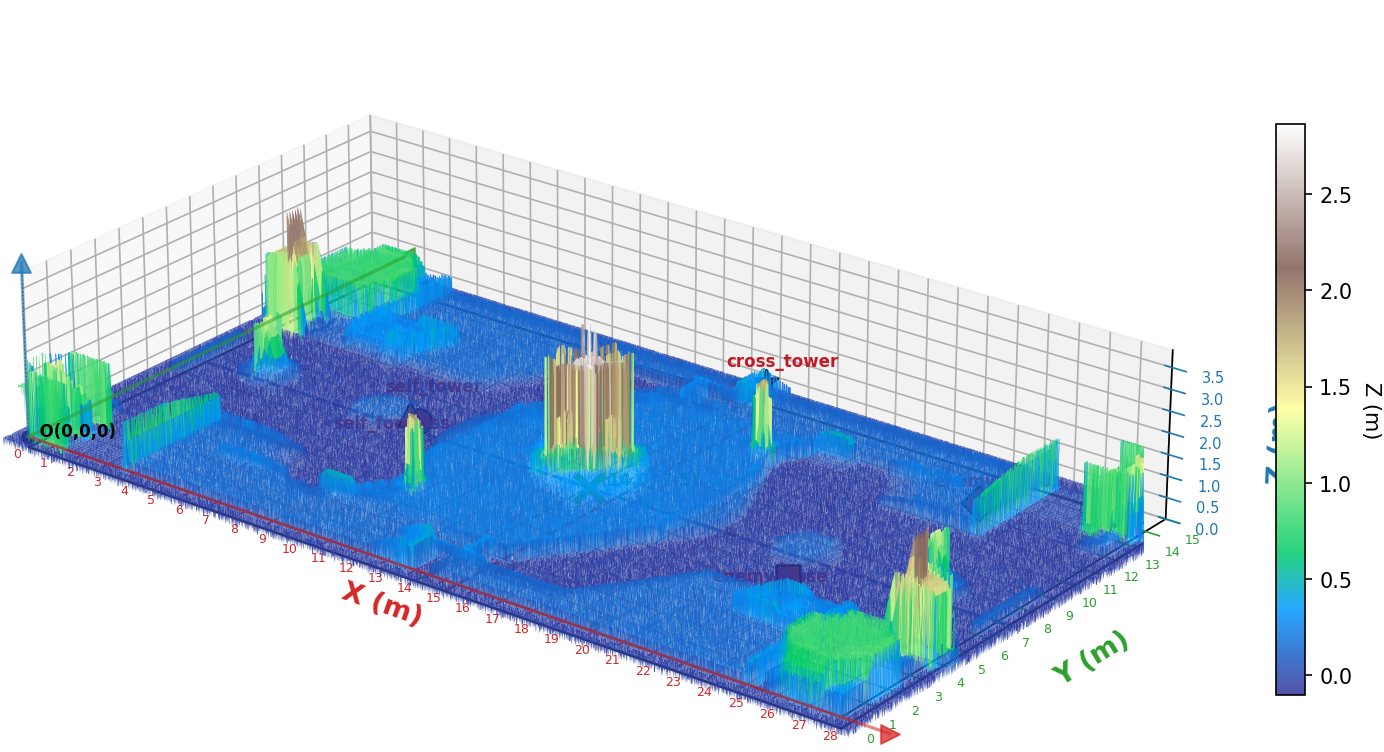
\includegraphics[width=0.72\textwidth]{figs/ground_height.png}
  \caption{场地扫描点云的地面高度分布（HeightGrid 网格高度的数据来源）。}
\end{figure}

\begin{figure}[H]
  \centering
  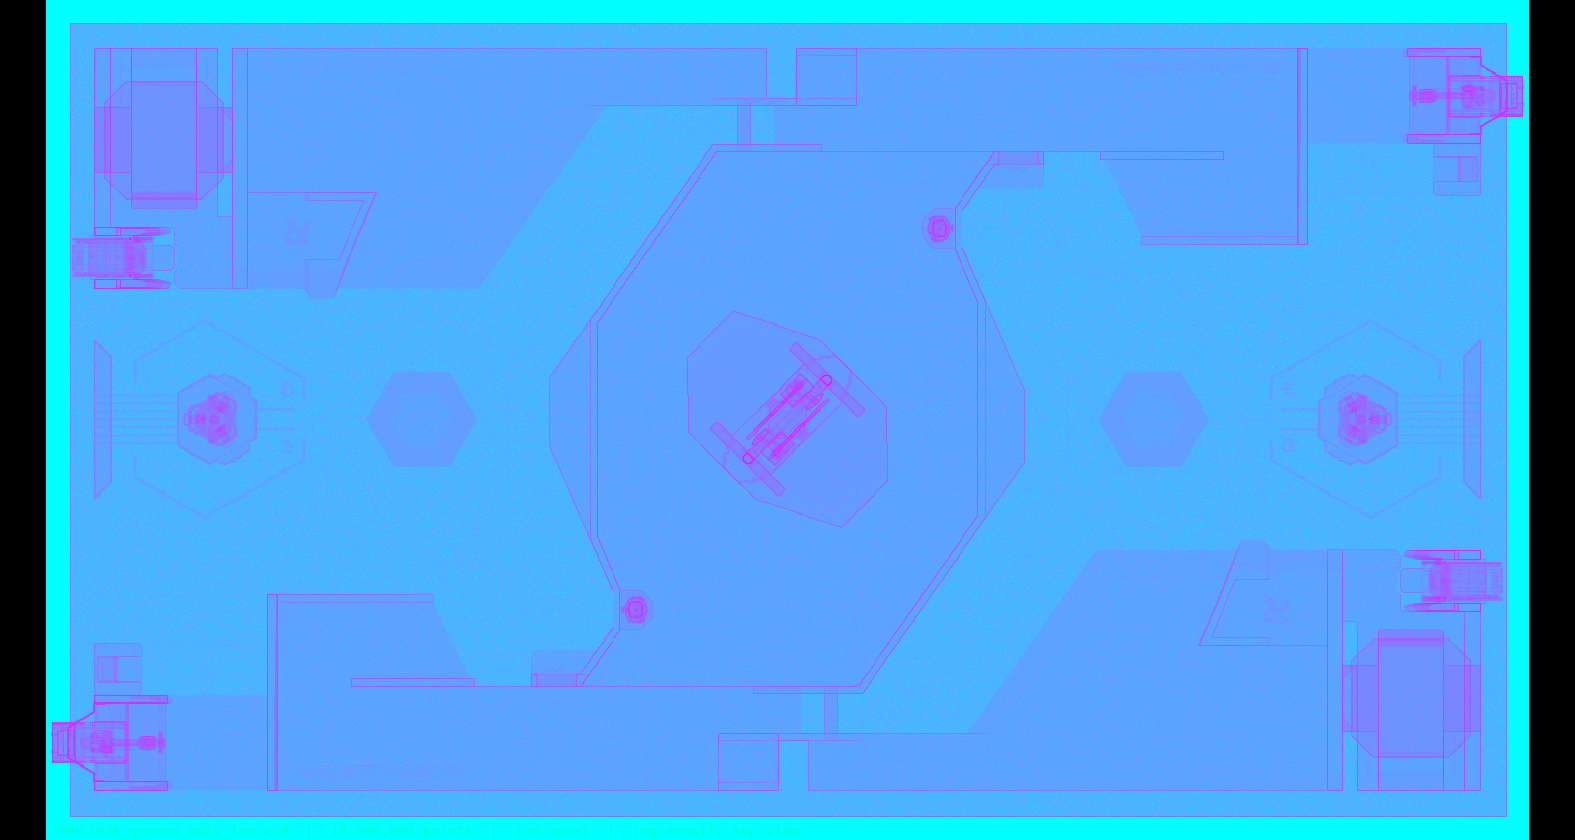
\includegraphics[width=0.62\textwidth]{figs/field_topview.png}
  \caption{RMUC 2026 场地俯视轮廓，用作配准与定位的场地地图。}
\end{figure}

\subsection{串口通信 radar\_serial\_node}
自主开发。发送：0x0305 小地图上传（敌我各 6 个坐标，48 字节，不超过 5Hz，坐标置 0 表示未发送；
标记精度规则为偏差 $<$0.8m 计 $+$1、0.8$\sim$1.6m 计 $+$0.5、$\ge$1.6m 计 $-$0.8）；
0x0301 与 0x0121 双倍易伤决策包（每局 2 次，每次 30 秒）。接收：0x0001/0003/0101/0105/020C/020E
解析后发布至 \code{/match\_info}（0x020C 为标记成功位，0x020E 的 bit0--1 为机会数、bit2 为激活状态）。
串口节点只负责数据转发，发送车辆数量由上游 detect 与 kalman 决定。

\subsection{可视化 debug\_map 与工具链}
debug\_map 增加盲区预测点显示；双倍易伤自动触发（机会数大于已触发数、场上存在有效标记且未激活时
自动发送 \code{/radar/decision\_request}，小地图窗口按 \code{v} 键可手动触发）。
工具链新增 Qt 控制面板 \code{rm\_control\_panel}（切换队伍、标定、录包）、
录包工具 \code{databag\_tool}（按场次自动命名保存至 \code{bags/}）。

\begin{figure}[H]
  \centering
  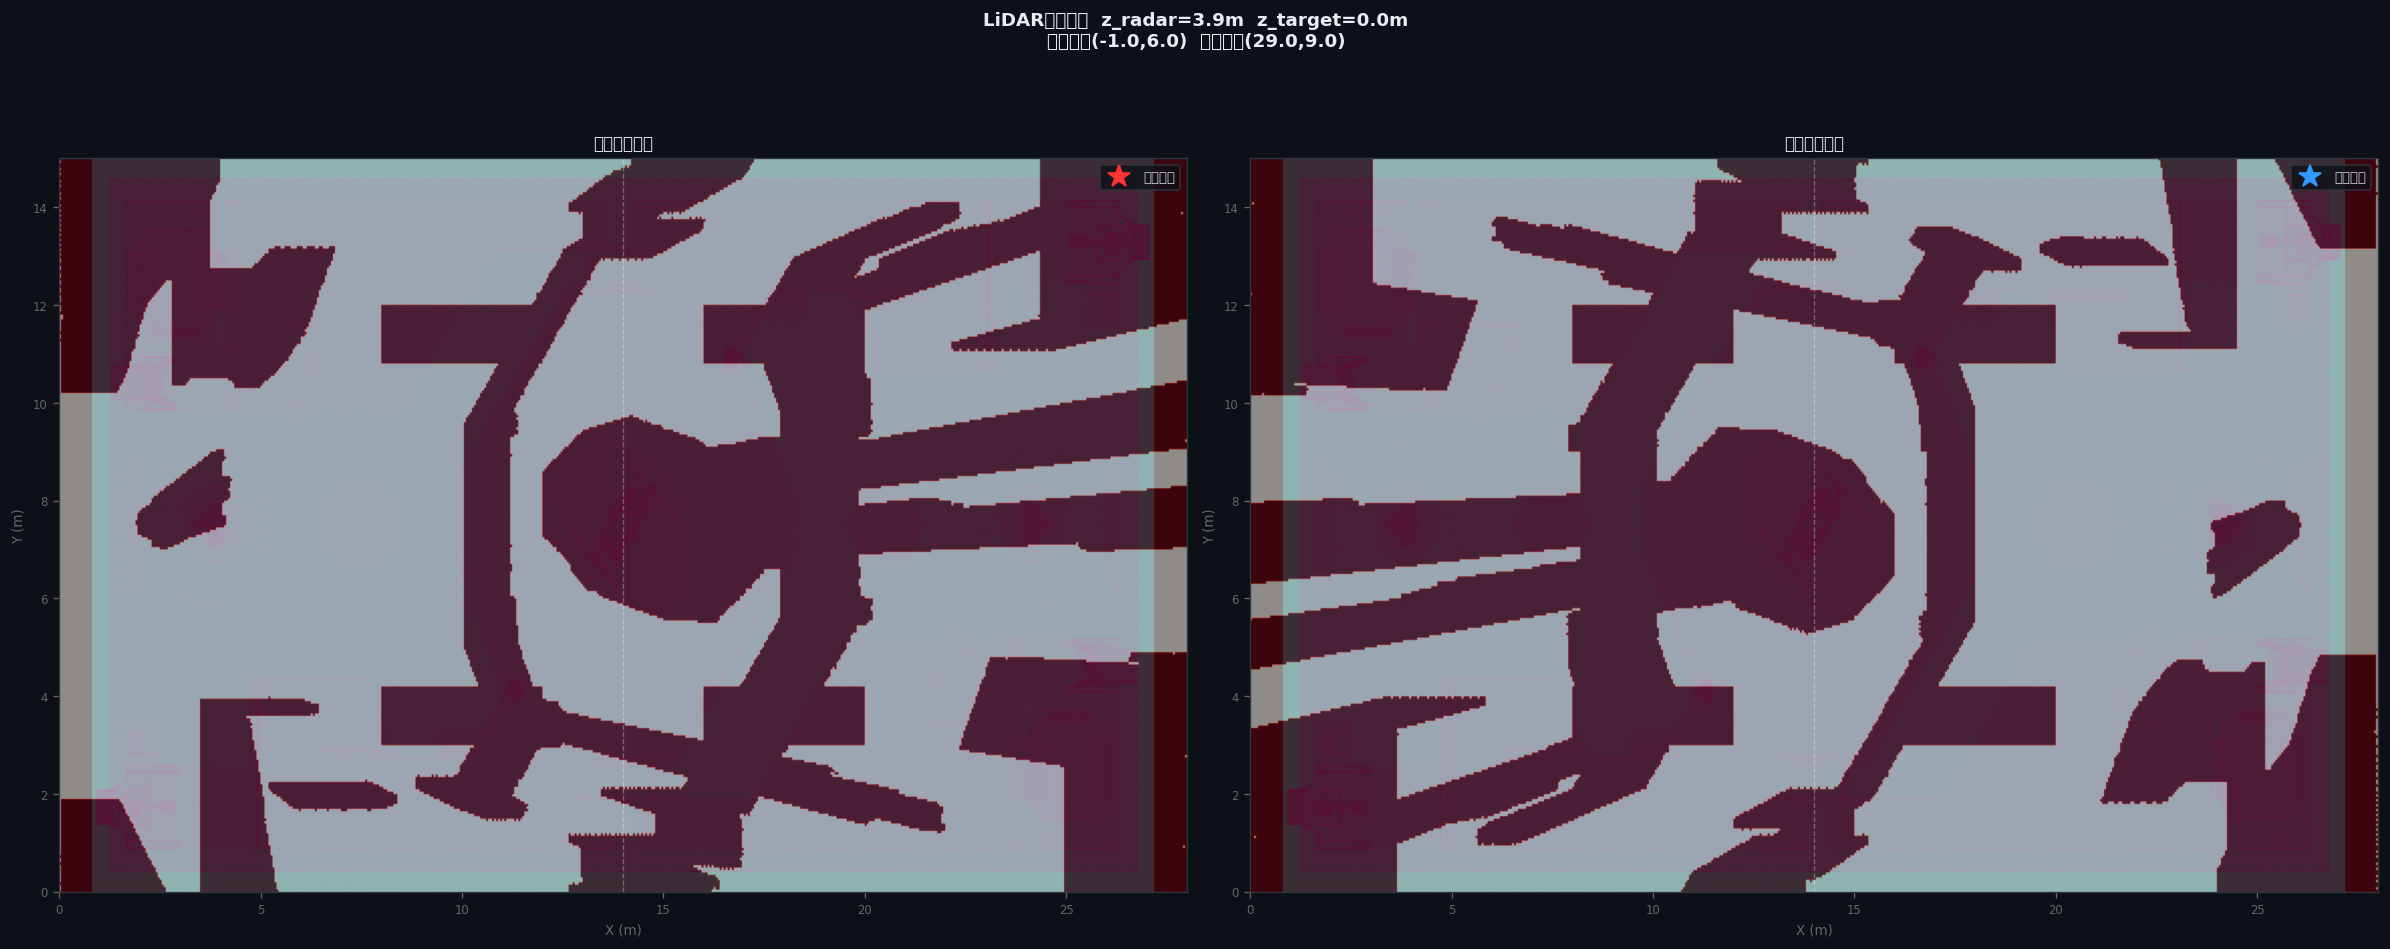
\includegraphics[width=0.95\textwidth]{figs/shadow_vis.png}
  \caption{雷达安装位置（高度 3.9m）对应的红蓝双方盲区可视化，盲区预测即针对图中深色区域。}
\end{figure}

%======================================================
\section{赛场应用效果}

区域赛于 5 月 19--24 日进行，正式局时长 7 分钟，共留存 9 局有效录制
（另有 5 月 21 日 10:02 的 75 秒短包与两个无法解析的损坏包未列入统计）。
局均易伤约 475 秒/局。统计口径：第五局起录包已含比赛阶段字段
（\code{game\_progress}），仅统计比赛进行时段（即 7 分钟局内，每局恰为 420s）；
前四局录包未含该字段，按整包统计（时长含局外时段，表中以 * 标注）。
使用 \code{tools/analyze\_vuln\_bag.py} 对全部 9 局统计：

\begin{table}[H]
\centering\small
\begin{tabularx}{\textwidth}{lcccccc}
\toprule
局次 & 开始时间 & 统计时长 & 平均发送车辆坐标数 & 发送 $\ge$3 辆时间占比 & 标记状态跳变 & 双倍易伤激活 \\
\midrule
第一局 & 5.20 12:12 & 651s$^{*}$ & 3.23 & 68\% & 0 & 0s \\
第二局 & 5.20 12:29 & 372s$^{*}$ & 2.26 & 29\% & 0 & 0s \\
第三局 & 5.21 21:15 & 525s$^{*}$ & 1.97 & 24\% & 0 & 0s \\
第四局 & 5.21 21:26 & 1335s$^{*}$ & 2.39 & 53\% & 0 & 0s \\
第五局 & 5.22 19:52 & 420s & 3.48 & 97\% & 26 & 0s \\
第六局 & 5.22 20:04 & 420s & 3.47 & 95\% & 32 & 0s \\
第七局 & 5.23 15:55 & 420s & 2.39 & 52\% & 23 & 0s \\
第八局 & 5.23 16:09 & 420s & 2.21 & 42\% & 23 & 0s \\
第九局 & 5.24 09:28 & 420s & 0$^{**}$ & 0\% & 30$^{**}$ & 0s \\
\bottomrule
\end{tabularx}
\caption{区域赛全部 9 局回放统计。$^{*}$前四局录包未含比赛阶段字段，统计时长为整包
（含局外时段）；$^{**}$第九局局内无车辆坐标发送数据（雷达基本未工作），标记状态跳变疑为
对局残留帧所致，不作有效计数。}
\end{table}

\begin{figure}[H]
  \centering
  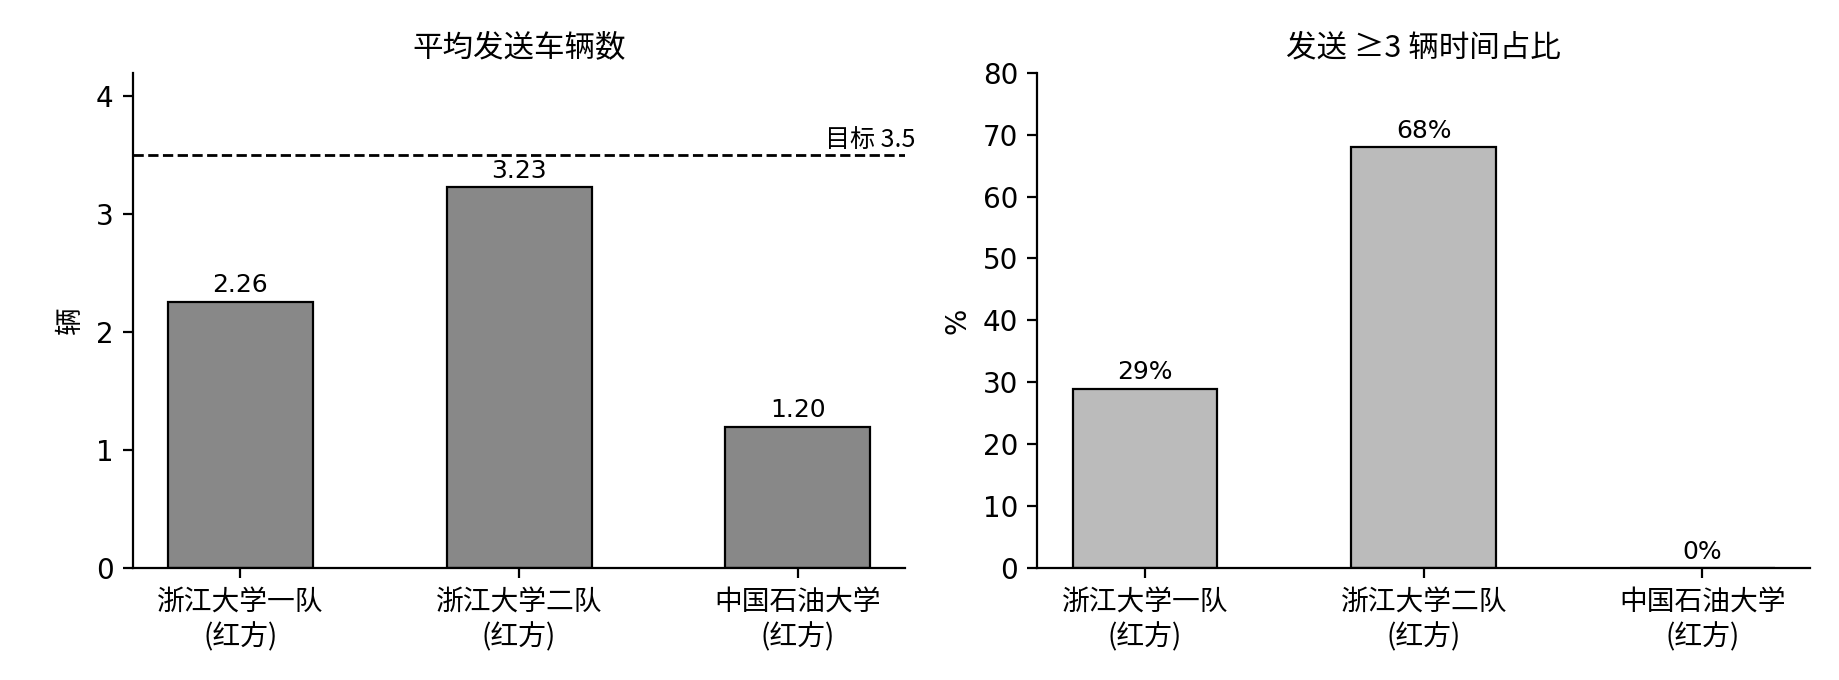
\includegraphics[width=0.9\textwidth]{figs/vuln_stats.png}
  \caption{各局局内平均发送车辆数与发送 $\ge$3 辆时间占比（依据回放统计结果绘制）。}
\end{figure}

\begin{figure}[H]
  \centering
  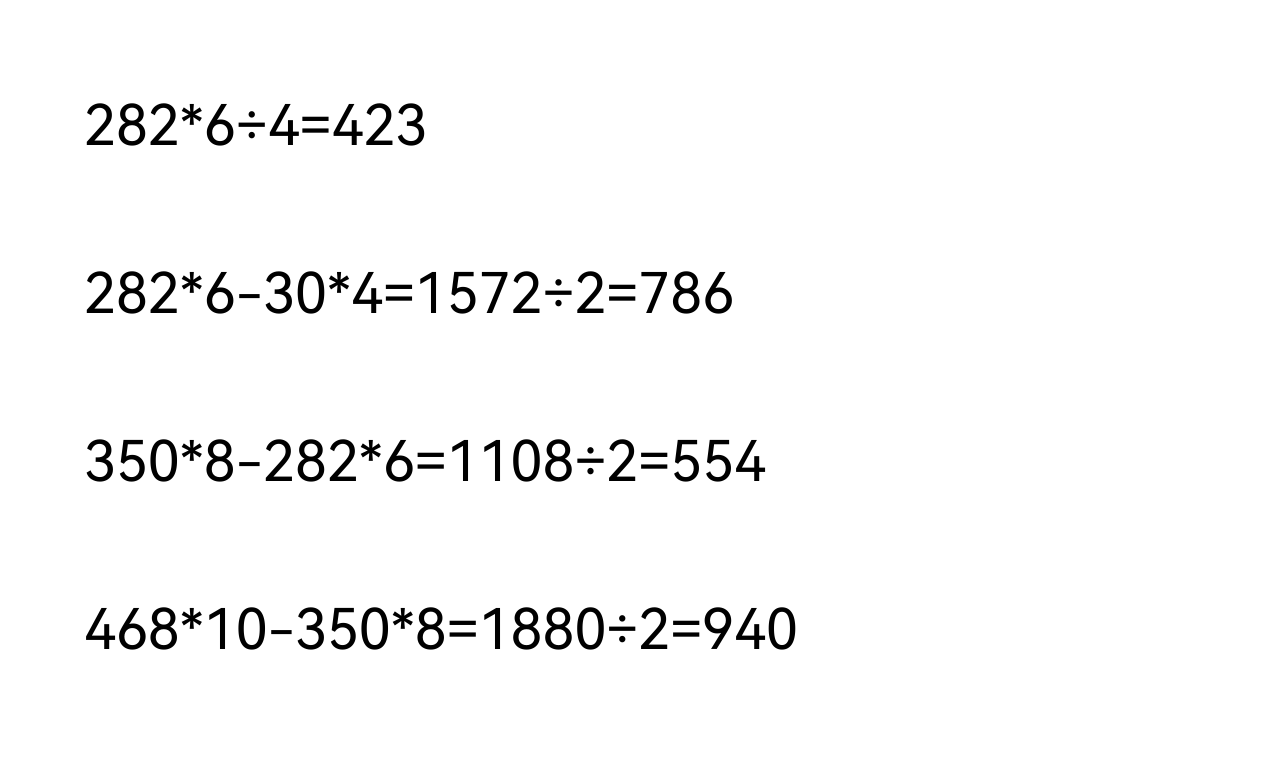
\includegraphics[width=0.7\textwidth]{figs/vuln_calc.png}
  \caption{部分场次局均易伤时长的计算手稿。}
\end{figure}

原因链条：\textbf{（1）}槽位填写时两车同号则后写覆盖先写，且无置信度仲裁；
\textbf{（2）}车辆可见但未识别出装甲板数字时整帧不发送；
\textbf{（3）}上述两条导致发送车辆坐标数偏低且波动大：第五、六局局内平均每帧发送
3.48/3.47 辆车的坐标（发送 $\ge$3 辆时间占比 97\%/95\%），第七、八局降至
2.39/2.21 辆（52\%/42\%），第九局雷达基本未发送车辆坐标数据；
\textbf{（4）}已发送坐标精度不足，偏差 $\ge$1.6m 按规则倒扣分数；
\textbf{（5）}第一至四局标记状态全程无跳变，机会数恒为 0；
第五局起标记状态出现 23$\sim$32 次跳变、机会数达到 2 次，但双倍易伤始终未激活；
\textbf{（6）}全部 9 局双倍易伤激活时长为 0 秒（此前统计到的 30 秒经核对全部发生在
准备阶段，为上一局的残留状态位，已剔除）。
根本原因在发送车辆数量与坐标精度，触发逻辑本身可用但受上游数据质量制约。

另有一局雷达未能正常启动，原因为 3 分钟准备时间内接线与配置未完成，且缺少强制赛前自检；
对策见 \code{docs/preflight\_check.md}。

%======================================================
\section{操作手赛后总结（原话记录）}

以下为 2026 赛季操作手赵书彤的赛后总结原话记录，仅修正笔误，未改变原有表述。
原话与回放统计结论的对应关系：``最多只会发 3 辆车的数据''与统计结果一致
（前四局局内平均每帧发送 1.97$\sim$2.39 辆车的坐标）；``双倍易伤完全没有开成''
与统计结果一致（9 局激活时长均为 0 秒）；``识别定位在回放中跑的时候是非常准的''
与``已发送坐标精度不足、偏差 $\ge$1.6m 按规则倒扣分数''的统计结论存在出入，
2027 赛季应利用回放包对发送坐标精度进行单独复判。

\begin{itemize}
  \item \textbf{效果自评：}``这个项目是我上场时候的代码，当然局均易伤只有 475 秒每局，
  属于很差的。由于红蓝不同，也导致局均易伤时长不同。应该是我们是红方的时候，
  整体的易伤时间会高出很多。''
  \item \textbf{双倍易伤：}``有一局，也就是两场，雷达因为完全没有开成，
  整个区域赛赛季由于我的代码问题，双倍易伤完全没有开成。''
  \item \textbf{问题定位：}``关于识别定位，我觉得我在回放中跑的时候是非常准的。
  我觉得最大的问题可能在通信的那个文件里面，那个的逻辑应该是有很大问题的，
  就是它可以通信，但是我感觉它同一时刻几乎最多只会发 3 辆车的数据，
  感觉是逻辑没有写好，平时测试的时候没有把这个问题放在心上。''
  \item \textbf{2027 赛季：}``27 赛季车少了一个应该问题不大了。注意一下重装的装甲板
  是否有变化，可能现在的不能直接用了。易伤的复判可以看一下我发的几个回放包，
  去查找问题。''
  \item \textbf{硬件配置：}``雷达硬件方面，利用现在的海康 CS060、6mm，以及自己的
  游戏本、Mid-70，我觉得这个配置已经很够用了，剩下来的只看你代码方面的完善了。''
  \item \textbf{购机说明：}``我的是 RTX4060 显卡，是惠普暗影精灵 10，内存是 1T。
  专门当时买了一个硬盘打 RM 的，但是当时硬盘刚涨价还不是非常贵。''
\end{itemize}

%======================================================
\section{2027 赛季注意事项}

\begin{enumerate}
  \item \textbf{车型变化}：机器人数量减少一个，需按新赛季规则手册修改 \code{robot\_slots.h}
        槽位表、\code{radar\_serial\_node.cpp} 协议映射、\code{armor\_class\_to\_slot} 映射与
        0x0003 血量表下标，修改后做全链路回放回归测试。
  \item \textbf{装甲板样式变化}：若样式有变化，\code{classify.onnx} 与 \code{armor\_yolo}
        可能无法直接适用，应尽早收集数据重新训练。
  \item \textbf{优先修复}：槽位同号覆盖；发送数据源改为 KF 轨迹直接输出，不依赖装甲板数字识别；
        增加置信度门控，坐标偏差过大时置零不发送。
  \item \textbf{流程规范}：赛前完整执行 \code{docs/preflight\_check.md}；用
        \code{tools/analyze\_vuln\_bag.py} 验证平均发送车辆数 $\ge$3.5、
        发送 $\ge$3 辆占比 $\ge$80\% 后方可上场。
\end{enumerate}

\end{document}
